Now that we've seen in part \ref{lbl:foxtarget} that the fox always runs towards some target. Furthermore, the rabbit perpetually runs towards its burrow. 

Therefore, we can say that a creature $C$ runs towards a target $T$ with a speed of $u$. We seek it's velocity in the $x$ direction ($v_x$) and in the $y$ direction ($v_y$).

\begin{figure}[h]
\centering
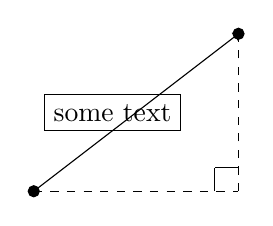
\begin{tikzpicture}
 
\draw[->] (-1,-1) -- (1.6,1);
\draw (1.3,-1) -- (1.3,-0.7);
\draw (1.3,-0.7) -- (1.6,-0.7);
\draw[dashed] (-1,-1) -- (1.6,-1);
\draw[dashed] (1.6,-1) -- (1.6,1);
\node[draw] at (0,0) {some text};

\filldraw [black] (-1,-1) circle (2pt);
\filldraw [black] (1.6,1) circle (2pt);
 
\end{tikzpicture}
\end{figure}